\chapter{Введение}

Тема транспортных проблем весьма популярна у исследователей, на нее написано огромное количество материала, о чем рассказано в книге \cite{gas}.

\section{Актуальность исследования}

Актуальность задачи состоит в том, что сама отрасль анализа дорожных данных стремительно развивается. Различные компании анализируют данные движения по дорогам. В городах проводятся все более массовые мероприятия. Таким образом, возникает необходимост оптимизировать эти процессы.

% 3 абзаца
\section{Цель и задачи исследования}
Модельный анализ пробелм, связанных с размещением

\section{Теоретические и методологические основы}
\section{Научная новизна}
\section{Практическая значимость}


\chapter{Теоретический обзор}

В этой главе обозревается литература и теории, которые могут быть полезны для цели исследования.

\section{Дизайн механизмов}


\section{Транспортное моделирование}
\section{Моделирование транспортных потоков как задача принятия решений}

Данный вопрос серьезно исследуется исследуется середины 50-х годов XX века.

Существует два типа моделей:
\begin{itemize}
	\item Микроскопические модели. Также --- модели-аналоги, так как вводится аналогия с газо- и гидродинамическими моделями. Такие модели используются для стратегичского планирования дорожной сети. В данной работе они рассматриваться не будут. 
	\item Микроскопические модели. В которых рассматриваются отдельные участники движения. Такие модели используются для решение локальных в территориальном смысле задач.
\end{itemize} \cite[225]{gas}

Модель строится в два этапа.

\begin{enumerate}
	\item Идентификация модели. В данном этапе определяются внешние параметры модели.
	\item Верификация. На этом уровне определяется адекватность построенной модели системе, которую она отражает.
\end{enumerate} \cite[225-226]{gas}

Поведенческие принципы агентов были сформулированы в работе \cite{wardrop}.



\begin{enumerate}
	\item Агенты независимо друг от друга выбирают маршруты своего следования, руководствуясь личными издержками.
	\item Агенты выбирают маршруты исходы из минимизации общих транспортных издержек сети.
\end{enumerate}

Это \textit{первый} и \textit{второй принципы Вардропа}.

В первом случае возникает конкурентное некоординированное равновесие, когда каждый действует исключительно в своих интересах. Это направление также встречается в литературе как эгоистическая маршрутизация (selfish routing) \cite[3]{rough2005}.

Допущения первого принципа:
\begin{itemize}
	\item Совершенная информированность участников движения о затратах по каждому возможному маршруту.
	\item Предполагается ничтожно малое влияние отдельного участинка на затраты по всем маршрутам.
\end{itemize}

Второй принцип Вардропа подразумевает централизованное управление дорожной ситуацией. Он также называется \textit{системной оптимизацией} \cite[26-27]{gas}. Ранее эти же принципы использовались в работах Найта \cite{knight} и 

Задача этого исследования относится к первому типу, однако интересно было бы рассмотреть ее и для второго типа. 


\section{Вероятность и стохастические процессы}

Вероятность --- мера, которая описывает результат повторяемого эксперимента, который не всегда точно воспроизводится. Если возможно представить, что эксперимент повторяется $N$ раз, вероятность определяется тогда как предел отношения благоприятных событий к числу экспериментов при $N\to\infty$.


\section{Стохастическое транспортное равновесие} \cite[316, Ю. Е. Нестеров, С. В. Шпирко]{gas}

\section{Игроки и сети} \cite[4]{GandN}

Рассмотрим конечное множество игроков $N = {1,...,n}$, которые объединены в сеть. 
Сеть --- это граф $(N, \mathbf{g})$, где $g$ --- сеть на множестве вершин $N$.
Вершины представляют структуру взаимодействия в игре, обозначая других игроков, чьи действия влияют на выигрыш конкретного игрока.

$\mathbf{g}$ может быть представлен как матрица смежности или как список пар соединенных вершин.


\section{Принципы моделирования загрузки}
\begin{itemize}
	\item Потокообразующие факторы
	\item Характеристики транспортной сети
	\item Поведенческие факторы (предпочтения при выборе способов передвижения)
\end{itemize}

Формализация этих факторов через граф.
Основа моделирования — математическая формулировка критерия, на основании которого агент выбирает способ передвижения. Этот критерий называется \textbf{обобщенной ценой пути}.

Исследования показывают, что время --- основной фактор, определяющий цену пути.\cite[4]{matmod_shvetsov}

Обобщенная цена может включать время передвижения, временные задержки, затраты, штрафы (используемые как меры управления).


\section{Теория очередей}


\section{Определения}
В постановке задачи мы используем терминологию, принятую в \cite[с. 461, Tim Roughgarden, Routing games]{agt2007}.
В этой книге взгляд с точки зрения дизайна механизмов.

\section{Цена анархии}
\cite{rough2001}
\cite{rough2005}

Вычисление цены анархии по \cite[69]{rough2005}.



\section{Одновременные игры}

Остановимся подробнее на одновременных играх. Их следует рассмотреть потому, что основная задача как раз и является одновременной игрой.




\section{Равновесие Нэша}

\section{Нормальная форма игры}
Игра в \textit{нормальной} (стратегической) форме состоит из:
\begin{enumerate}
	\item Списка \textit{игроков} $N$;
	\item Множества \textit{стратегий} для каждого игрока;
	\item Профиля \textit{выигрышей} (платежей) для каждого профиля стратегий.
\end{enumerate}

\section{Парадоксы транспортного равновесия}
\subsection{Пример Пигу}\cite[447]{agt2007}
Задача схожа с примером Пигу, рассмотренным в книге \cite{agt2007}.

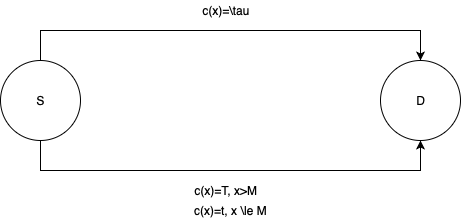
\includegraphics[scale=.7]{img/pigou}


\subsection{Парадокс Браесса}\cite[65]{gas}

\section{Трагедия общих ресурсов \footnote{англ. Tragedy of commons}}

Есть $n$ игроков, каждый из которых претендует на часть трафика $x_i\in[0,1]$.

Если общий трафик $\sum_j x_j$ превышает пропускную спопобность канала, то никто не выигрывает.
Если
$\sum_j x_j < 1$,
тогда выигрыш $u_i$ игрока 
$i$ составляет $x_i(1-\sum_j x_j)$

Найдем равновесные стратегии в этой игре.
Рассмотрим игрока $i$ и зафиксируем стратегии других игроков: $t=\sum_{j\ne i} x_j<1$.

Тогда игроку $i$ необходимо решить задачу оптимизации. 
Его выигрыш будет составлять в зависимости от $x$:
$u(i)=x(1-t-x)\to max$, который достигается при $x=(1-t)/2$.

Если все будут устремлять свой интерес к максимуму, то возникнет ситуация $\forall i: x_i=(1-\sum_{j\ne i} x_i)/2$, в силу симметричности которой $x_i=1/(n+1)$.

Эта ситуация является <<трагедией>> в силу того, что выигрыш каждого игрока мал: $u_i=1/(n+1)^2$, а сумма выигрышей всех игроков $u=n/(n+1)^2\approx 1/n$. Если ограничить общий трафик, например, $1/2$, то общий выигрыш уже будет $1/4$, что в $n/4$ раза больше\cite[5]{agt2007}.


\chapter{Задача о парковочных местах}

\section{Постановка задачи}
\setstretch{2}

Существует $M$ парковочных мест.

В игре участвуют $N$ игроков, $N >> M$.

$\tilde N$ --- количество севших за руль

$(N - \tilde N)$ --- количество поехавших общественным транспортом.

Издержки игроков $c(x)$:
\begin{itemize}
 \item  $t$, если $\tilde N\le M$,
 \item  $T$, если $\tilde N>M$;
 \item  $\tau$, альтернативный маршрут,
 \item  $t<\tau<T$
\end{itemize}

$\tau$ — альтернативный маршрут.
Сравнить его с лотереей ${t,T}$.
$P(t)$ задается $\tilde N$: $P=\frac{M}{\tilde{N}}$ (or $1$, if $M \le \tilde N$).

\textbf{Чистое равновесие}: $\frac{M}{\tilde N}t+(1-\frac{M}{\tilde{N}})T\approx\tau$.


$\tilde{N}$ (количество севших за руль) : $\frac{M}{\tilde{N}}t+(1-\frac{M}{\tilde{N}})T\le\tau$.

${N-\tilde N}$ (кто едет транспортом) : $\frac{M}{(\tilde{N}+1)}t+(1-\frac{M}{\tilde{N}+1})T\ge\tau$.

$T-\tau = \frac{M}{\tilde{N}}(T-t)$

$\tilde{N}=[\frac{M(T-t)}{T-\tau}]$ — чистое равновесие. Но «так не бывает», ибо неясно, кто эти счастливчики.

$p$ — вероятность сесть за руль.

$Q$[тебе достанется место] такова, что $\tau = Qt+(1-Q)T \Rightarrow Q(T-t)=T-\tau$, $Q*=\frac{T-\tau}{T-t}$.

Но! $Q$ должно быть вычислено как функция от $p$!

\setstretch{2.5}
$(1-p)^{N-1} + \\ (N-1)p(1-p)^{N-2} + \\ C_{N-1}^2 p^2(1-p)^{N-2} + ... + \\ C_{N-1}^{M-1}p^{M-1}(1-p)^{N-M} + \\ C_{N-1}^{M}p^M(1-p)^{N-M-1}(\frac{M}{M+1}) + \\ C_{N-1}^{M+1}p^{M+1}(1-p)^{N-M-2}(\frac{M}{M+2}) + \\ p^{N-1}\frac{M}{N} = \\ Q^*$

Решить как обратную функцию, найти $p^*$ — решение $p^*(\frac{T-\tau}{T-t})$.

\textbf{Гипотеза:} в равновесии $Np^* >> M$.



\setstretch{1.2}

\bigskip

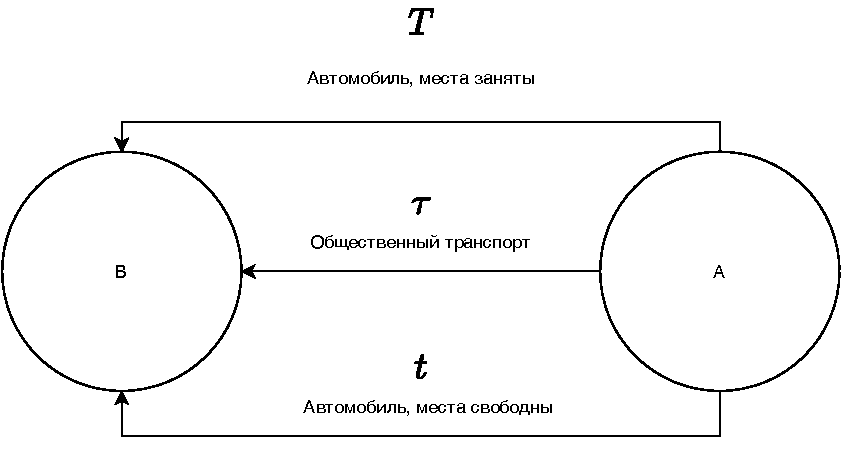
\includegraphics[scale=0.8]{img/task_scheme}


\section{Общее решение}

\inputpython{../code/task1.py}{1}{41}
% Введение, формальные сведения

\subsection{Вариации}

Для $N=1000$:

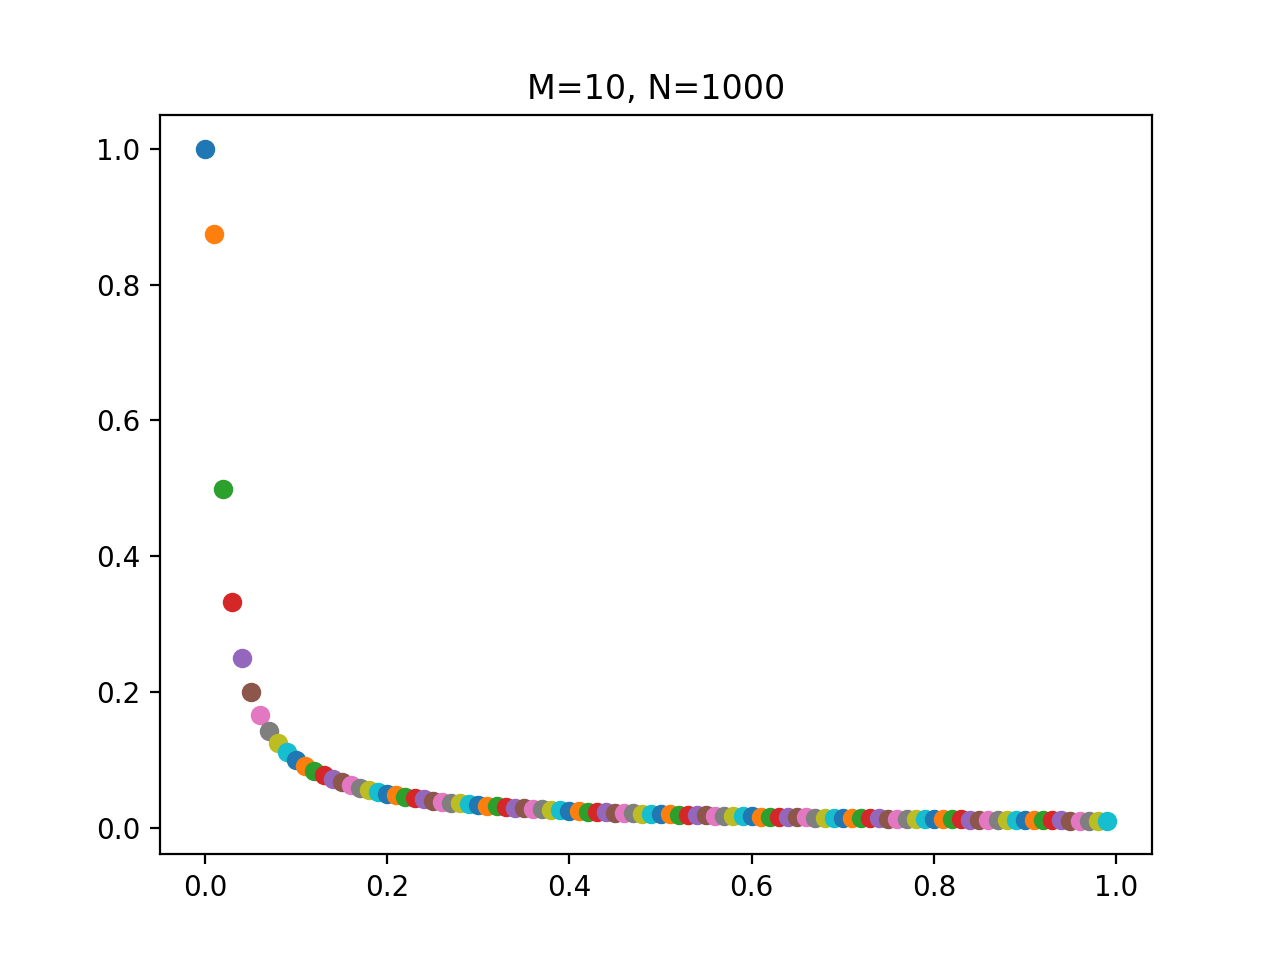
\includegraphics[scale=0.5]{img/1000_10}
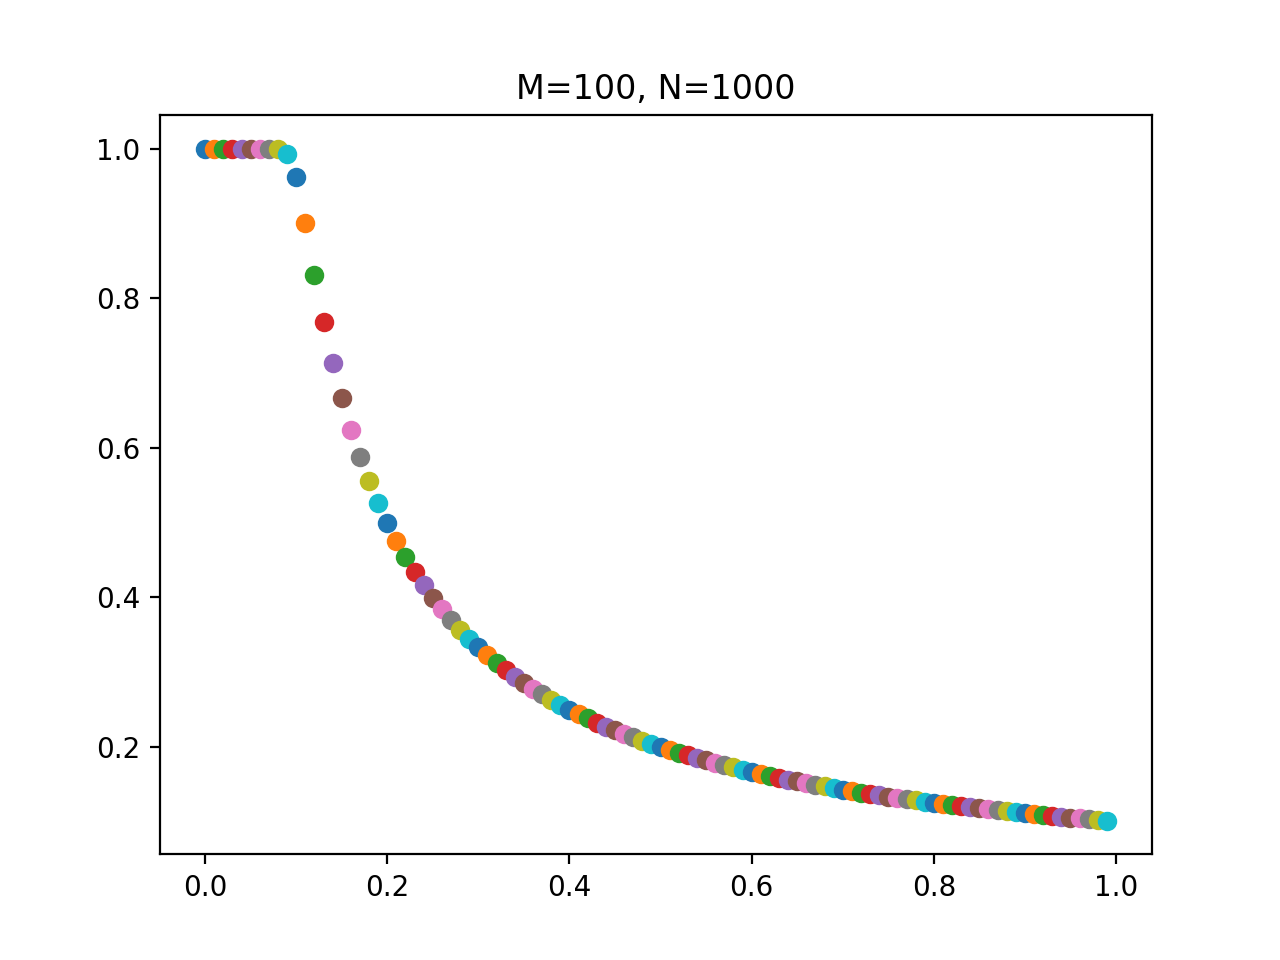
\includegraphics[scale=0.5]{img/1000_100}
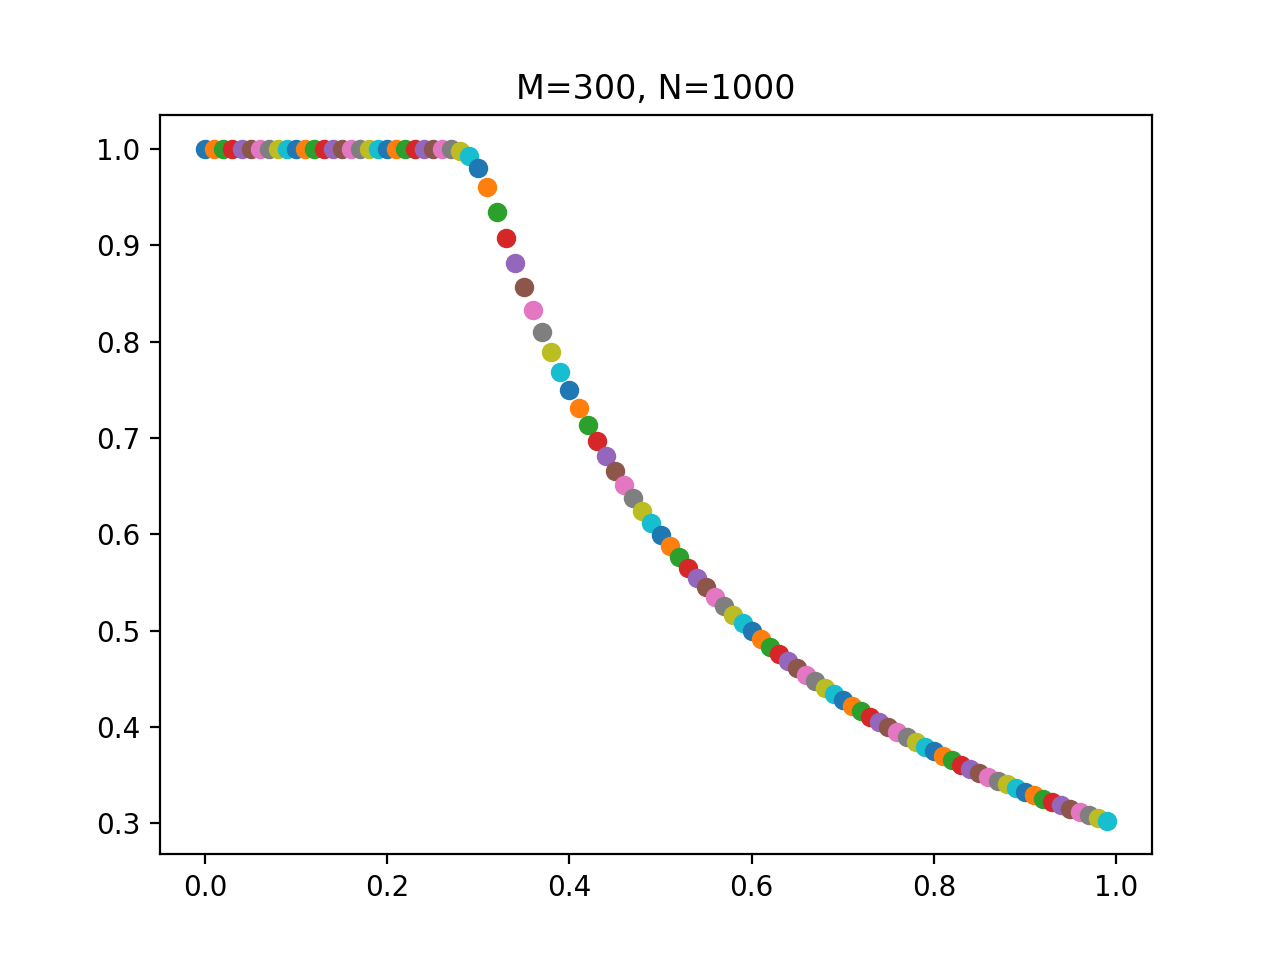
\includegraphics[scale=0.5]{img/1000_300}
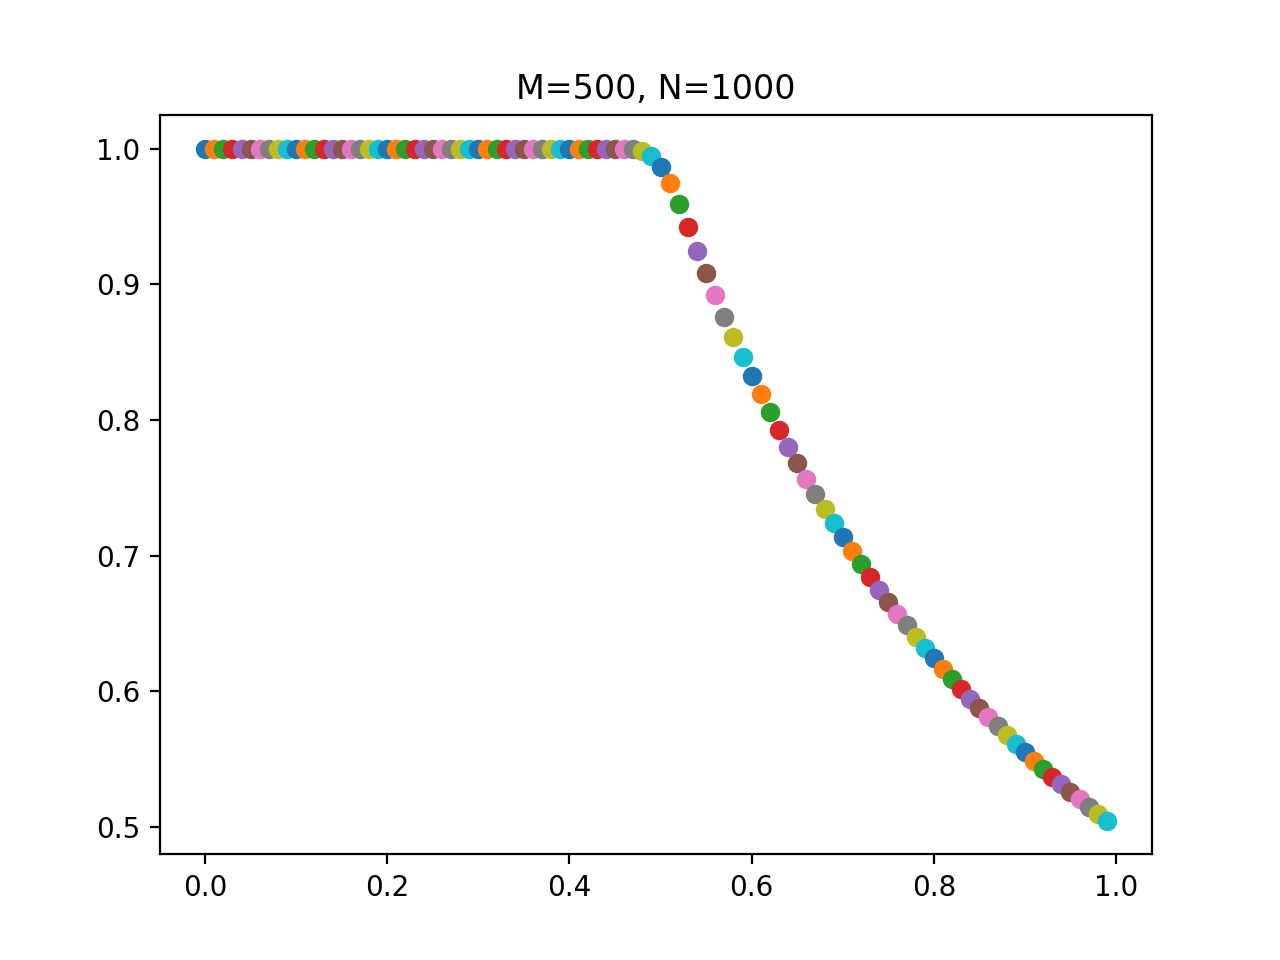
\includegraphics[scale=0.5]{img/1000_500}
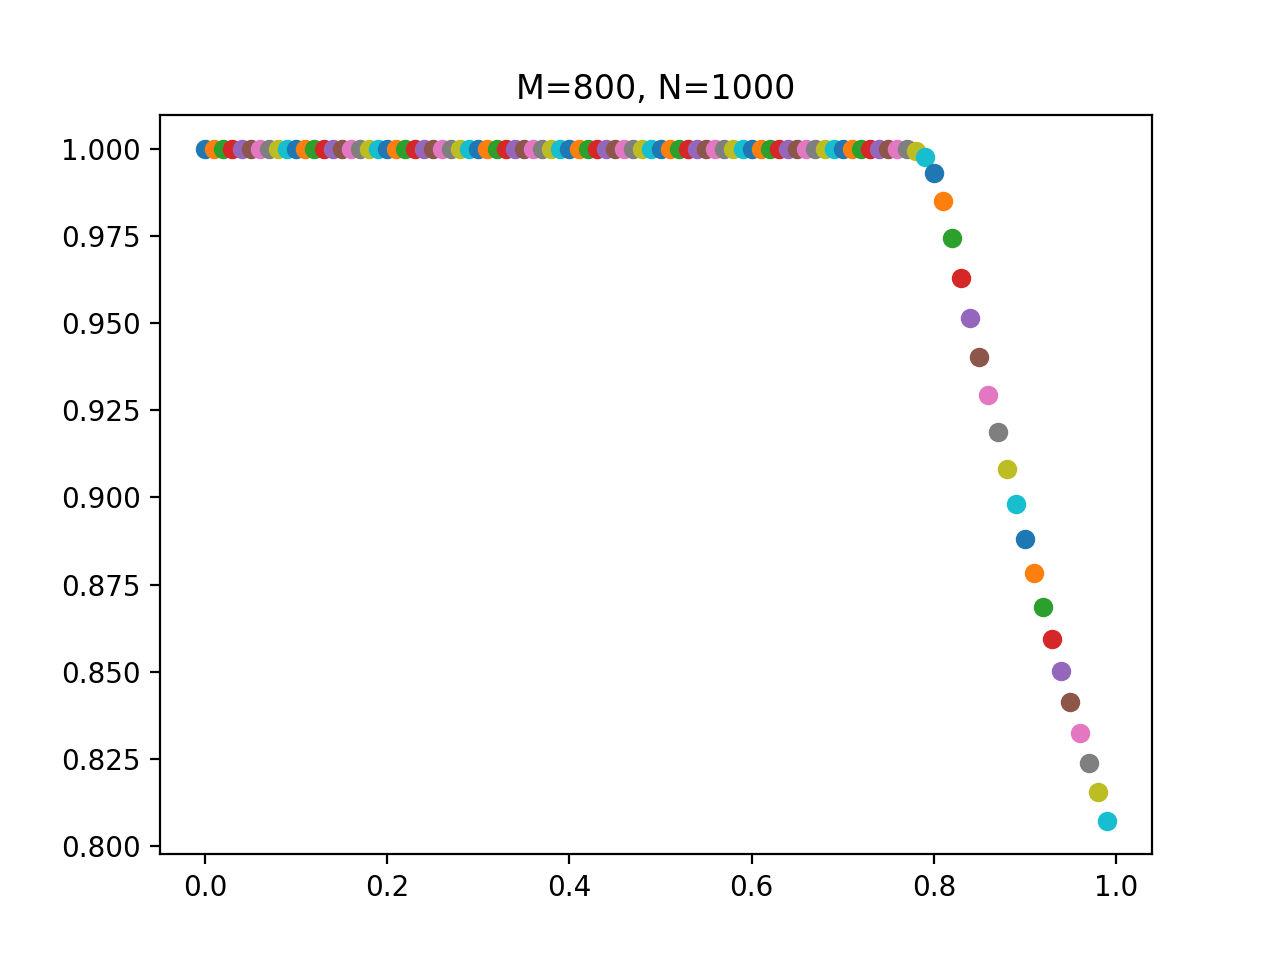
\includegraphics[scale=0.5]{img/1000_800}
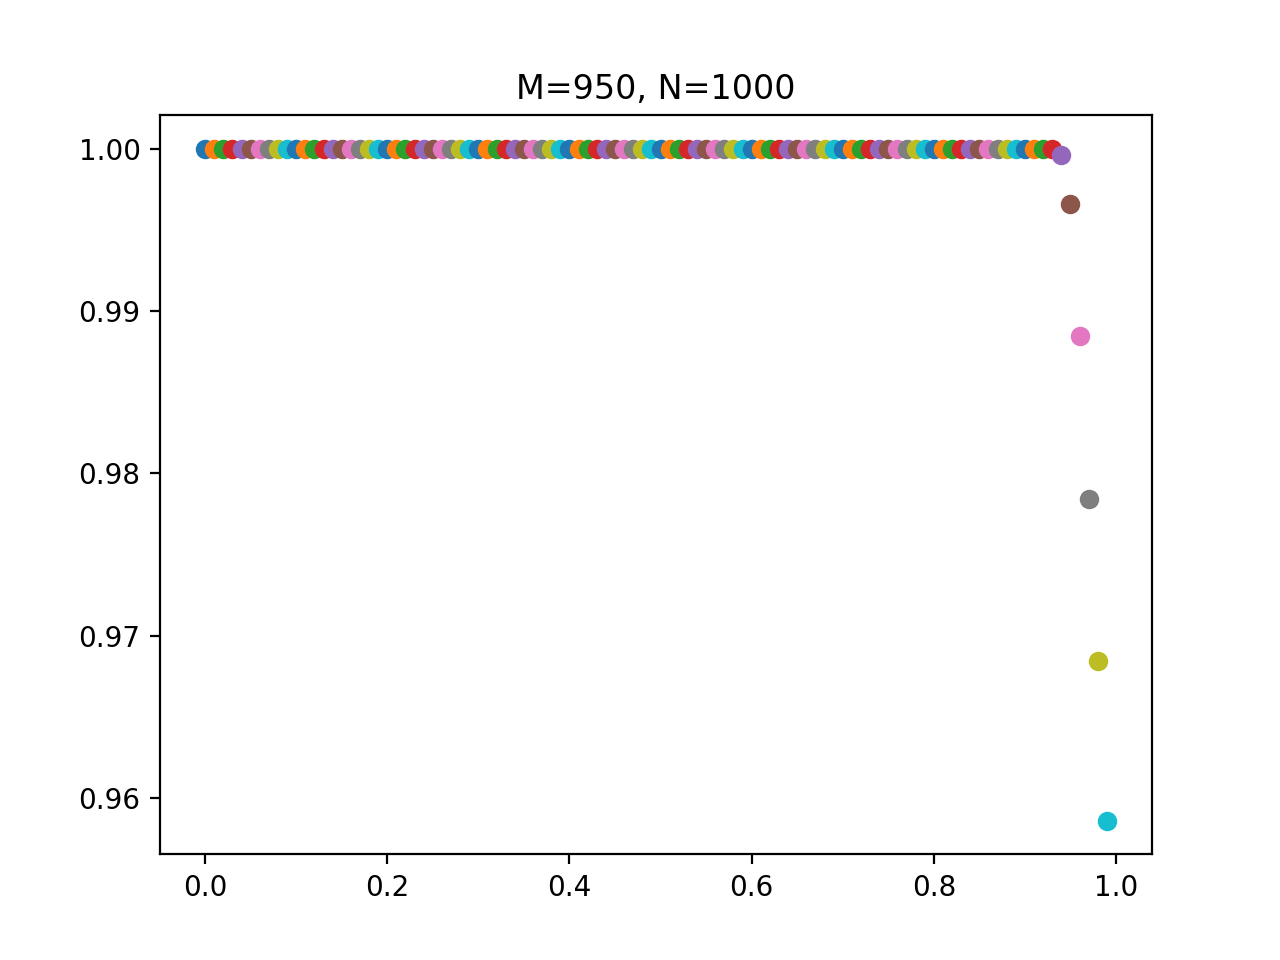
\includegraphics[scale=0.5]{img/1000_950}
\skip
Для $N=100$:

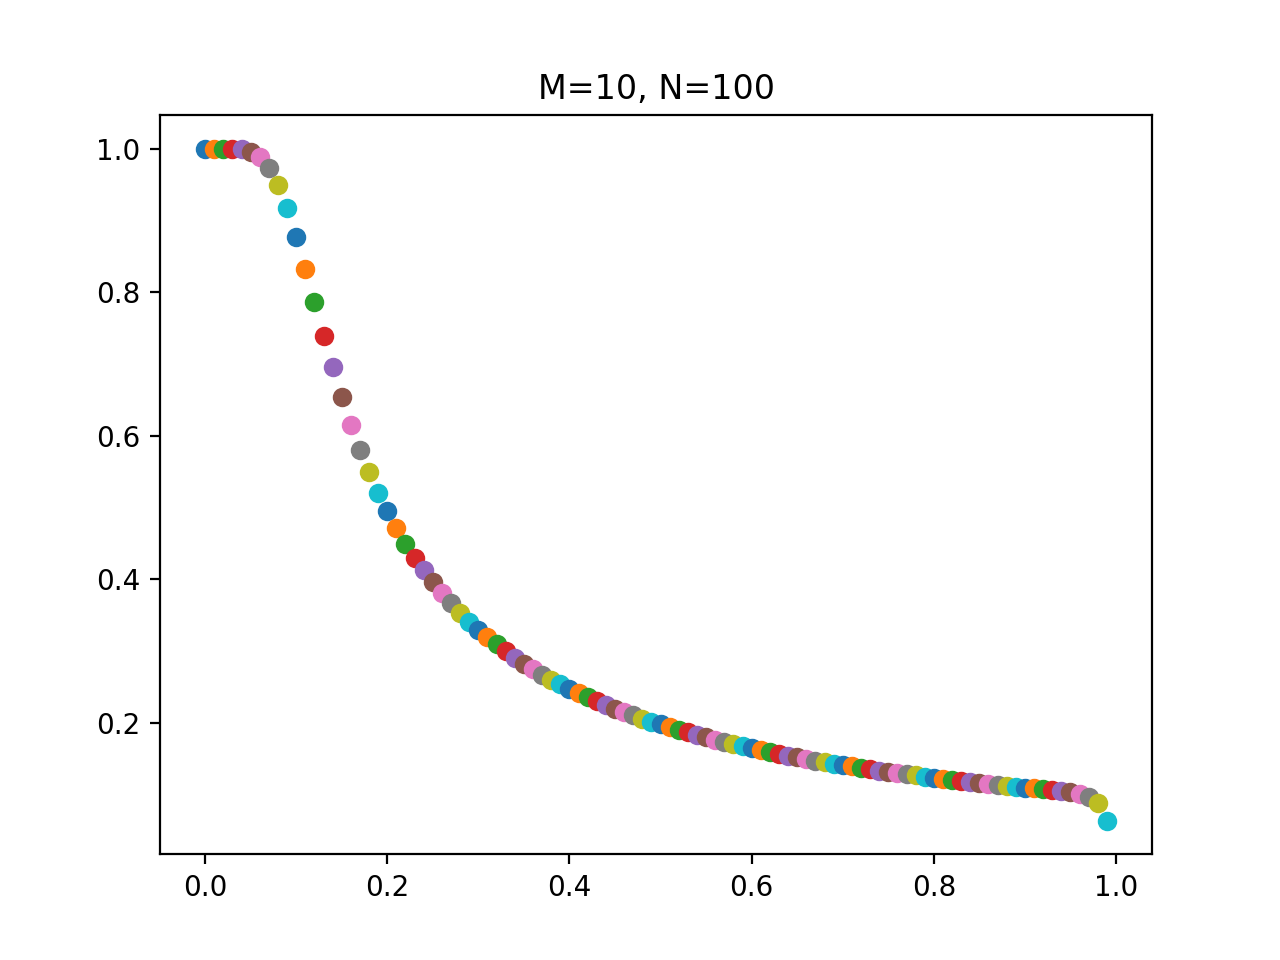
\includegraphics[scale=0.5]{img/100_10}
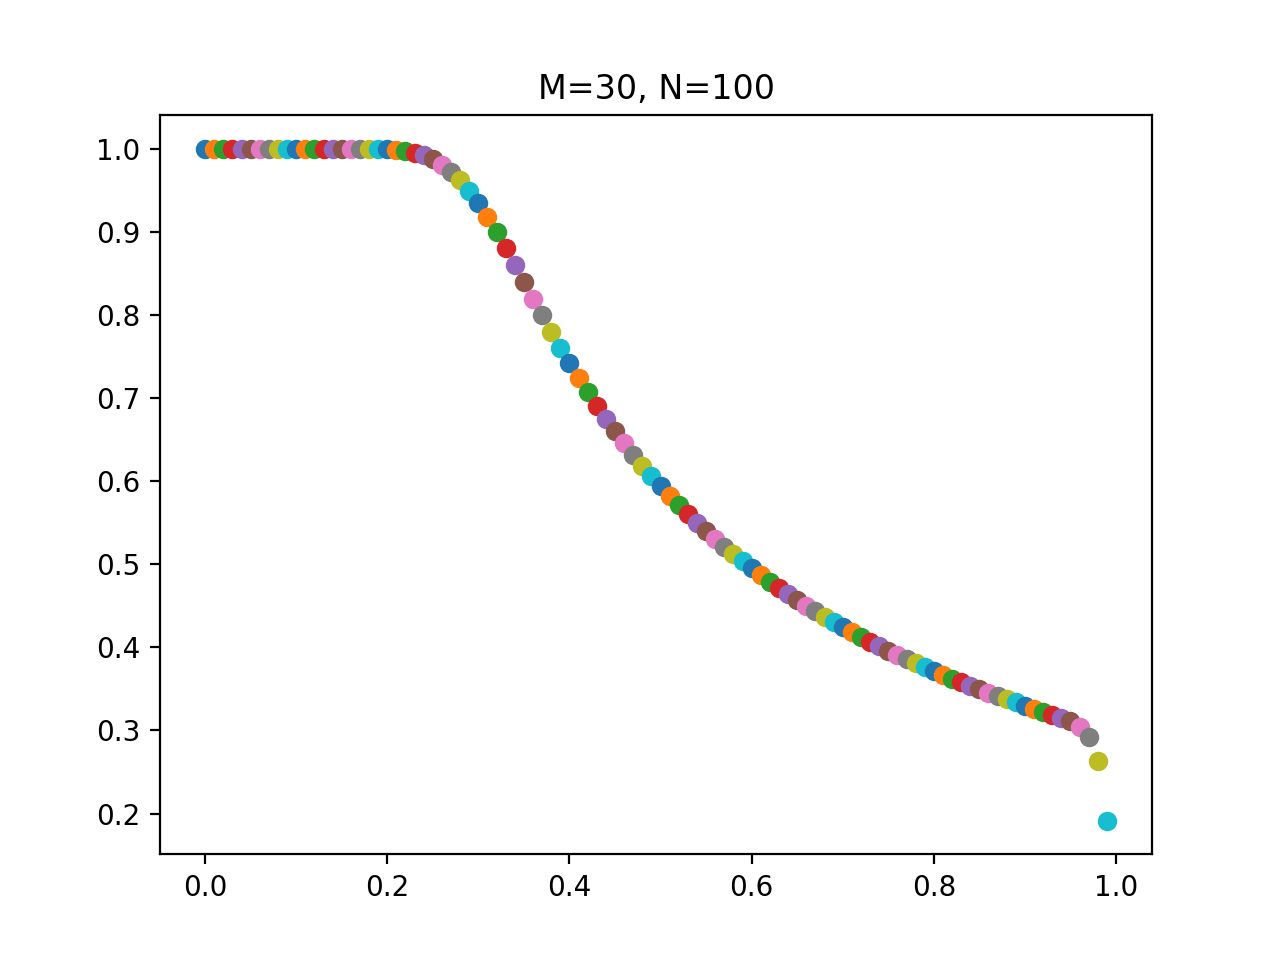
\includegraphics[scale=0.5]{img/100_30}
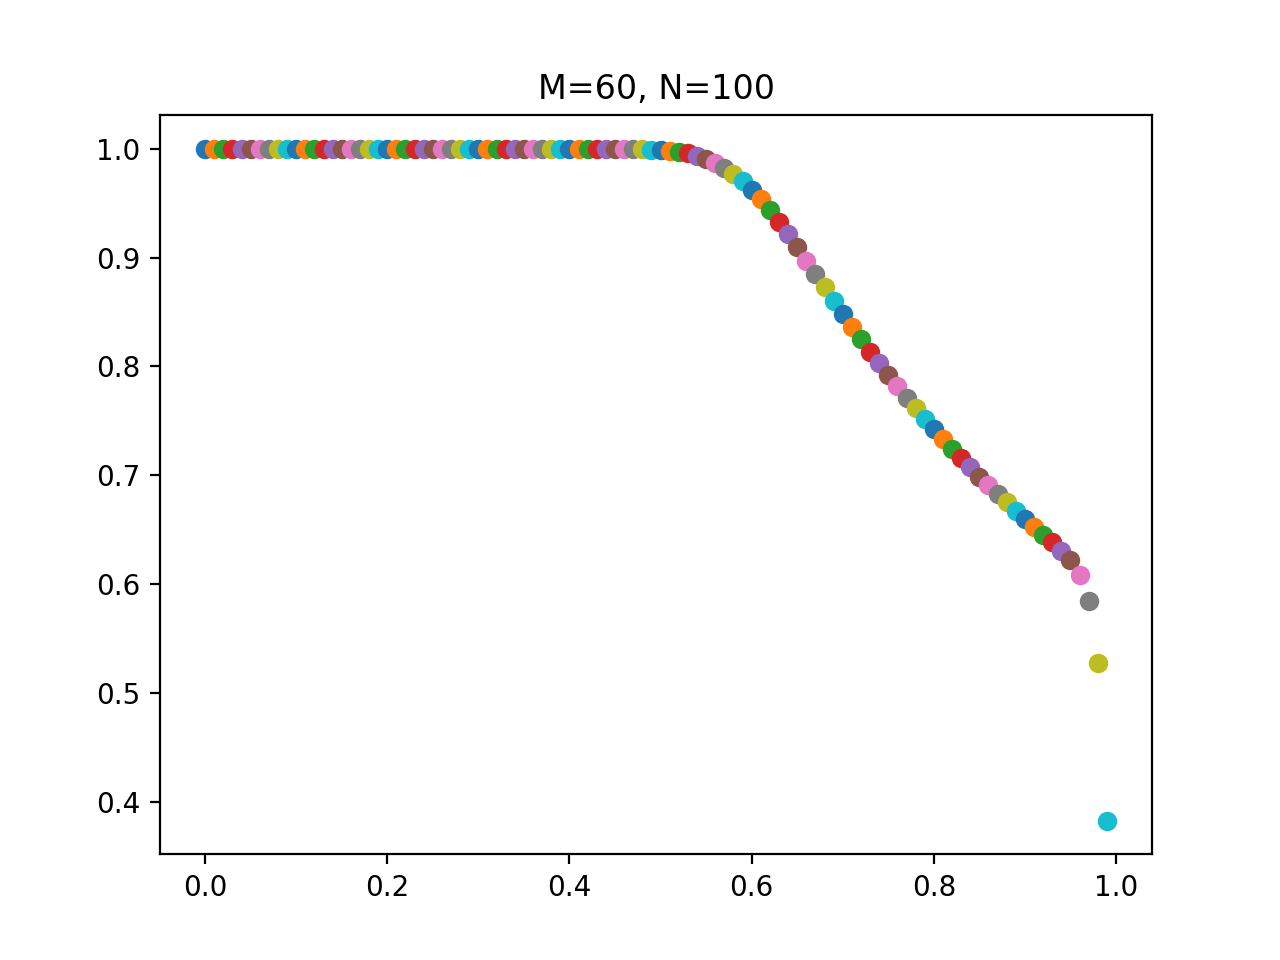
\includegraphics[scale=0.5]{img/100_60}
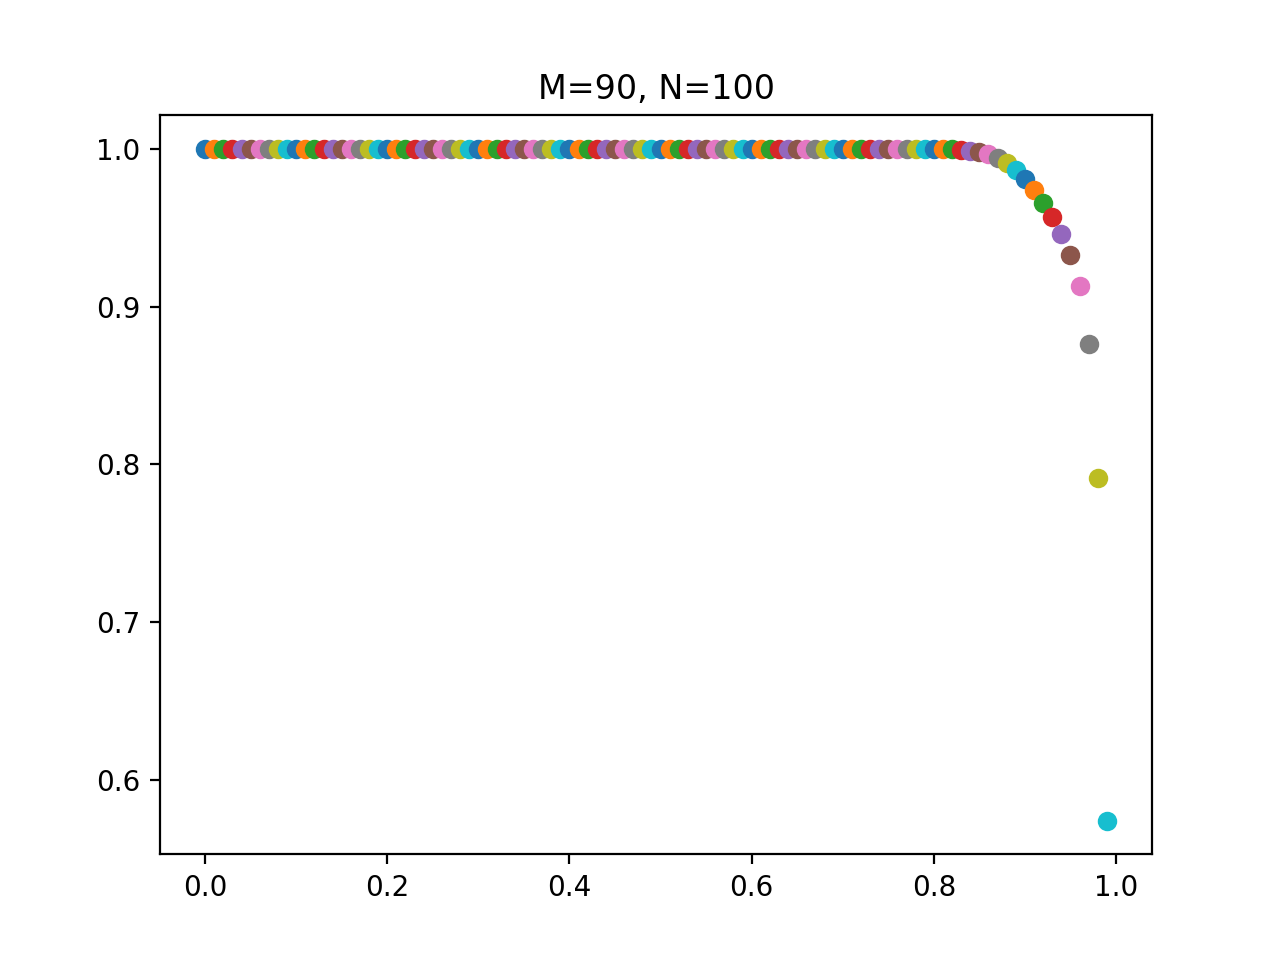
\includegraphics[scale=0.5]{img/100_90}

\section{Подсчет задачи на примерах из жизни}

Варианты с разными параметрами. Подставим некоторые реальные данные:

\subsection{СК <<Олимпийский>> (Москва)}

\begin{itemize}
	\item Количество парковочных мест: $700$ \footnote{Источник: https://carparkings.ru/parkovki/moskva/parkovka-u-sportivnogo-kompleksa-olimpijskij.html}.
	\item Максимальная вместимость: $35 000$ зрителей
	\item Максимальная вместимость после реставрации: $10 000$ \footnote{Источник: https://ru.wikipedia.org/wiki/Олимпийский}
\end{itemize}
$0,02$ в старой конфигурации
$0,07$ после реставрации

\subsection{Крокус Сити холл (Москва)}
\begin{itemize}
	\item Максимальная вместимость зала: $7233$
	\item Парковка $6000$ \footnote{Источник: https://crokus-hall.com/about/}
\end{itemize}

$0,83$

\subsection{Альберт-холл (Лондон)}

\subsection{Москва-сити}
\begin{itemize}
	\item Количество парковочных мест $10 500$  \footnote{Источник: http://moscow-city-towers.ru/parking.php}
	\item Посещаемость в день:  $175 000$ \footnote{Источник: https://moscow-city.online/news/34113/}
\end{itemize}

0,06

\subsection{Филармония (г. Майкоп)}
\begin{itemize}
	\item Мест в партере: $612$ \footnote{Источник: http://filarmoniya-ra.ru/interiors}
	\item Мест на парковке: $48$ \small{(посчитано по спутниковой карте)}
\end{itemize}
\begin{figure}
	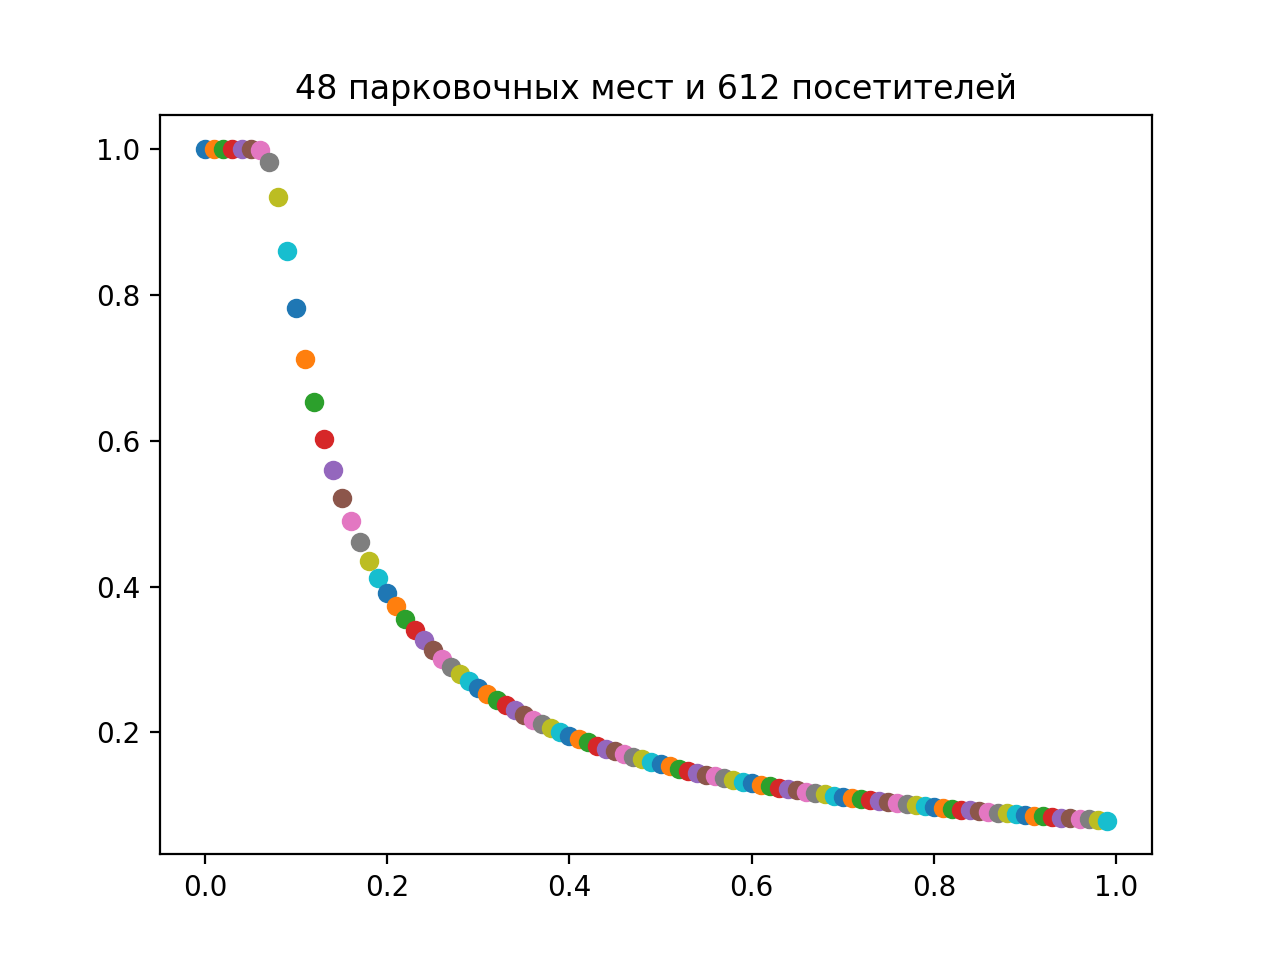
\includegraphics[scale=0.6]{img/612_48}	
\end{figure}

\begin{figure}
	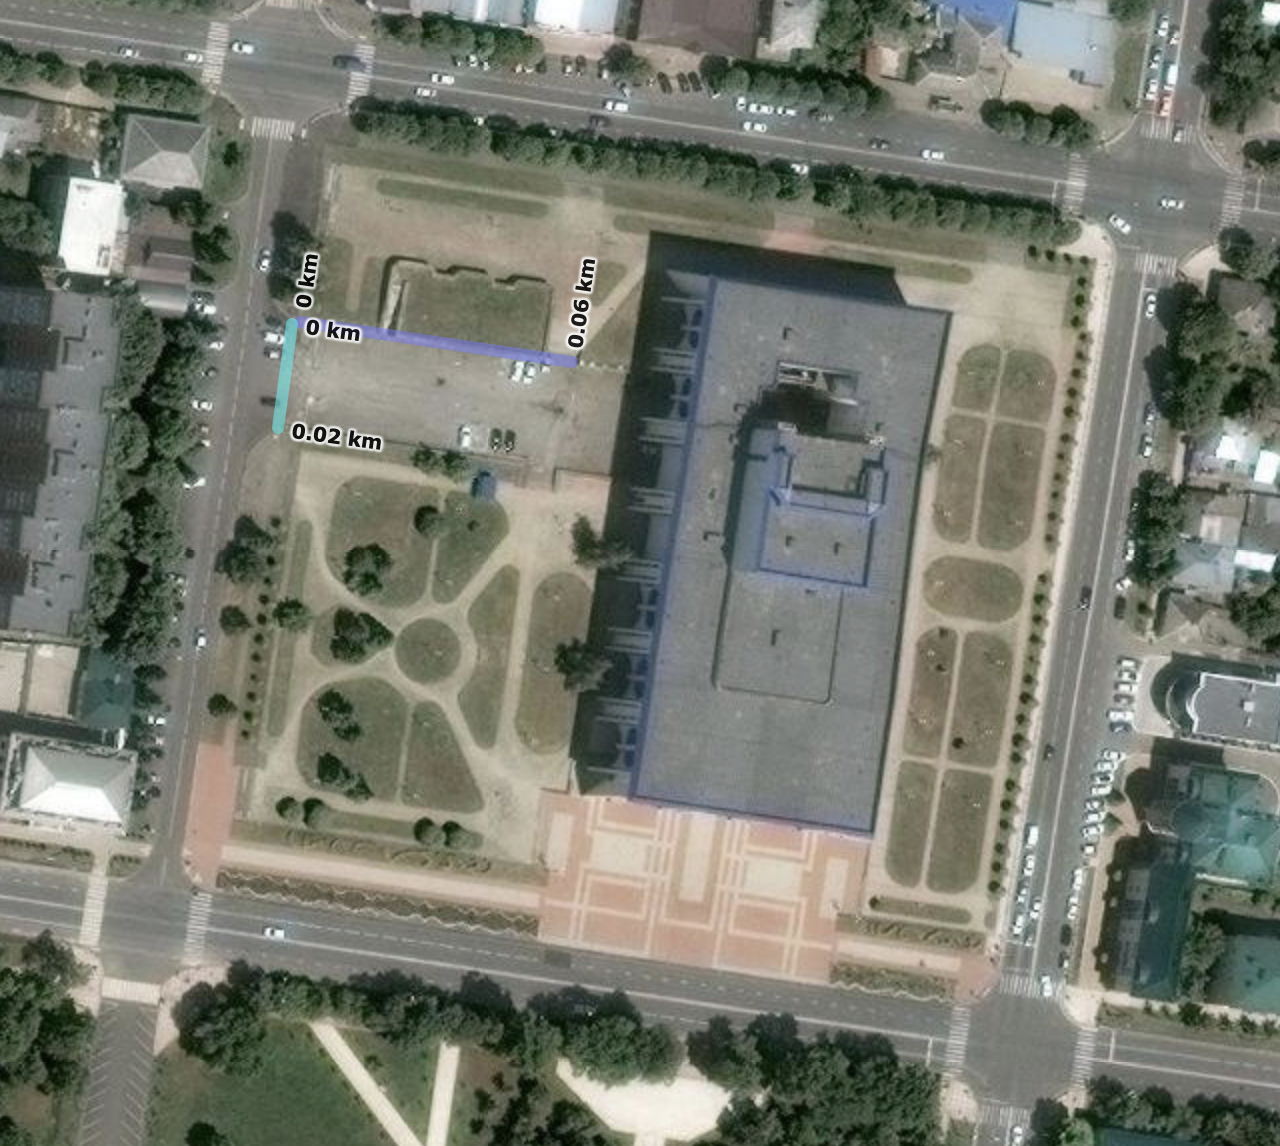
\includegraphics[scale=0.3]{img/filarmony_parking}
	\caption{Майкопская филармония на спутниковых Яндекс-картах}
\end{figure}

0,07


%\footnote{Предположим, что в Майкоп приехал Николай Басков, и все билеты раскуплены}


%\section{Рассуждения на тему задачи}

\section{Другие подходы к проблеме}
Транспортный поток как физическая материя, состоящая из молекул \cite[168]{lukanin}
\section{Варианты практического решения}
Ценовое регулирование




\chapter{Выводы исследования}

\begin{itemize}
	\item Разработана модель ...
	\item В процессе анализа...
	\item В ходе ...
\end{itemize}
% Давно известно, что...
% Анализ, проведенный в гл... показывает, что ...
% Прикладная задача
% Решение прикладной задачи методами программмирования
% Применение в жизни
% Коммерческое применение...
% И, наконец, последний вывод...
